% =====================================================================
%  THE LUNAR HEAT-FLOW STUDY: A GUIDEBOOK FROM THE GROUND UP
%
%  A self-contained textbook companion to the manuscript
%  "Difference of Lunar Regolith Thermal Conductivity K_d at the
%   Apollo 15 and 17 Heat-Flow Boreholes."
%
%  Written for a reader with NO prior background. It builds every idea
%  from scratch -- the physics, the equations and how they are used,
%  the data, the computer model, and the statistics (bootstrap, MCMC,
%  AICc) -- before arriving at the results.
%
%  Build on Overleaf: upload the whole primer/ folder, compile
%  guidebook.tex with pdfLaTeX. Every figure lives in primer/figures/.
% =====================================================================
\documentclass[11pt]{report}

\usepackage[a4paper,margin=2.5cm]{geometry}
\usepackage[T1]{fontenc}
\usepackage{lmodern}
\usepackage{microtype}
\usepackage{amsmath,amssymb}
\usepackage{graphicx}
\usepackage{booktabs}
\usepackage{xcolor}
\usepackage[most]{tcolorbox}
\usepackage{caption}
\captionsetup{font=small,labelfont=bf,labelsep=period}
\usepackage[hidelinks,colorlinks=true,linkcolor=teal!60!black,
            urlcolor=teal!60!black]{hyperref}
\usepackage{enumitem}
\setlist{itemsep=2pt,topsep=3pt}
\linespread{1.05}

\definecolor{teal}{HTML}{2A7E7E}
\definecolor{coral}{HTML}{C0573B}

% chapter heading: lighter than the book-class default
\usepackage{titlesec}
\titleformat{\chapter}[display]
  {\normalfont\huge\bfseries\color{teal!55!black}}
  {\chaptertitlename\ \thechapter}{14pt}{\Huge}
\titlespacing*{\chapter}{0pt}{0pt}{18pt}

% callout boxes
\newtcolorbox{plainbox}[1][]{colback=teal!5!white,colframe=teal!60!black,
  boxrule=0.6pt,arc=2pt,left=6pt,right=6pt,top=4pt,bottom=4pt,
  fonttitle=\bfseries,title={In plain words},#1}
\newtcolorbox{mathbox}[1][]{colback=coral!5!white,colframe=coral!55!black,
  boxrule=0.6pt,arc=2pt,left=6pt,right=6pt,top=4pt,bottom=4pt,
  fonttitle=\bfseries,title={The equation, term by term},#1}
\newtcolorbox{keybox}[1][]{colback=yellow!8!white,colframe=orange!55!black,
  boxrule=0.6pt,arc=2pt,left=6pt,right=6pt,top=4pt,bottom=4pt,
  fonttitle=\bfseries,title={Key takeaway},#1}

\title{\vspace{-1cm}\bfseries The Lunar Heat-Flow Study:\\
A Guidebook from the Ground Up}
\author{A plain-language companion to\\
\emph{``Difference of Lunar Regolith Thermal Conductivity $K_d$ at the
Apollo 15 and 17 Heat-Flow Boreholes''}}
\date{\today}

\begin{document}
\maketitle
\thispagestyle{empty}

\begin{plainbox}[title={Who this book is for}]
You. Even if you have never taken a physics or statistics course. Every
chapter starts from zero and builds up. The coloured boxes are your
friends: \textcolor{teal!60!black}{\textbf{plain-words}} boxes restate
the idea simply, \textcolor{coral!55!black}{\textbf{equation}} boxes
unpack every symbol of a formula, and
\textcolor{orange!60!black}{\textbf{key-takeaway}} boxes summarise what
to remember. You can read the whole thing skipping every equation box
and still understand the study; the boxes are there for when you want to
go deeper.
\end{plainbox}

\tableofcontents

% =====================================================================
\part{Foundations}

\chapter{Why anyone studies heat in the Moon}

The Moon looks dead and unchanging, but just under its surface there is a
slow, quiet flow of heat --- and that flow carries information we can get
no other way.

\paragraph{The surface vs.\ the inside.}
The Moon's surface is baked by the Sun during its two-week-long day and
freezes during its two-week night. But a metre below the surface, none
of that daily drama is felt. Down there, the temperature is set by two
things only: how well the soil conducts heat, and a faint warmth seeping
up from the Moon's deep interior. Measuring that quiet underground
temperature tells us about both.

\paragraph{The number we are chasing.}
The single most important property of the soil, for this purpose, is its
\textbf{thermal conductivity}: how easily heat passes through it. We
write it $K$, and the specific value deep down (where the soil is packed
and settled) is $K_d$ (``$d$'' for deep). Lunar soil is an
extraordinary insulator --- several times better than the styrofoam in a
coffee cup --- which is exactly why the daily heat wave cannot get far
below the surface.

\paragraph{Why it matters in practice.}
Today, scientists who model the Moon use \emph{one single value of $K_d$
for the entire globe}. That value was never checked against direct
underground measurements, because such measurements exist at only two
spots in all of history: the Apollo 15 and Apollo 17 landing sites,
where astronauts buried thermometers in 1971--72. Every spacecraft that
infers ground properties from orbit, and every future mission that wants
to ``see'' below the surface, leans on that one assumed number.

\begin{keybox}
This study uses the only two underground temperature records ever taken
on the Moon to test a hidden assumption everyone relies on: \emph{is one
conductivity value good enough for the whole Moon?} The short answer we
will build toward: no --- the two sites differ by roughly a factor of
two, and that difference is real.
\end{keybox}

% =====================================================================
\chapter{How heat moves: conduction from scratch}

\section{Heat flows downhill (in temperature)}
Heat is just jiggling atoms. Where atoms jiggle a lot, it is hot; where
they jiggle little, it is cold. When a hot region touches a cold region,
the jiggling spreads out: heat always flows from hot to cold. This
spreading-through-solid-material is called \textbf{conduction}
(Figure~\ref{fig:conduction}).

\begin{figure}[t]
\centering

\includegraphics[width=0.92\linewidth]{figures/fig_book_conduction.pdf}
\caption{\textbf{Conduction.} Heat flows from the hot end to the cold
end of a bar. How fast it flows depends on two things: how good a
conductor the material is ($K$), and how steep the temperature change is
along the bar. A steeper change, or a better conductor, means more heat
per second.}
\label{fig:conduction}
\end{figure}

\section{Fourier's law: the rate of heat flow}
How much heat flows is captured by a 200-year-old rule, Fourier's law.
In words: the heat flowing through a surface equals the conductivity
times the steepness of the temperature change across it.

\begin{mathbox}
\[
q \;=\; -\,K\,\frac{\partial T}{\partial z}
\]
\textbf{$q$} is the heat flux --- how much heat crosses one square metre
each second (watts per m$^2$). \textbf{$K$} is the conductivity.
\textbf{$\partial T/\partial z$} is the temperature gradient: how fast
temperature $T$ changes as you move in depth $z$ (it is just ``rise over
run'' for the temperature-vs-depth line). The minus sign encodes ``heat
flows from hot to cold'' --- toward lower temperature.
\end{mathbox}

\begin{plainbox}
Think of a crowded room emptying through a door. The flow of people ($q$)
is bigger if the door is wide (large $K$) and if the crowd is much denser
inside than outside (steep gradient). Heat behaves the same way.
\end{plainbox}

\section{From a single rule to the heat equation}
Fourier's law tells us the flow \emph{through one surface}. To track the
temperature \emph{everywhere over time}, we apply one more idea:
bookkeeping. For any thin slice of soil, the heat that builds up inside
it equals the heat flowing in from one side minus the heat flowing out
the other. Combine that bookkeeping with Fourier's law and you get the
\textbf{heat equation} --- the master equation of this whole study.

\begin{mathbox}
\[
\underbrace{\rho\,c_p\,\frac{\partial T}{\partial t}}
  _{\text{heat piling up in the slice}}
\;=\;
\underbrace{\frac{\partial}{\partial z}\!\left(K\,\frac{\partial T}{\partial z}\right)}
  _{\text{(heat in)} - \text{(heat out)}}
\]
\textbf{Left side:} how fast the slice's temperature rises
($\partial T/\partial t$), times how much heat that takes ---
\textbf{$\rho$} is density (how much stuff is packed in) and
\textbf{$c_p$} is specific heat (how much energy to warm it by one
degree). \textbf{Right side:} the net heat arriving by conduction ---
Fourier's law applied on both faces of the slice. If more heat comes in
than leaves, the slice warms; if balanced, it holds steady.
\end{mathbox}

\begin{keybox}
The heat equation just says: \emph{temperature changes because more heat
flows into a place than out of it.} Everything the computer does is solve
this one equation, over and over, for the lunar soil column.
\end{keybox}

% =====================================================================
\chapter{The lunar setting: skin, depth, and the steady zone}

\section{Two sources of heat}
The soil column is heated from both ends (Figure~\ref{fig:heatflow}a).
From \emph{above}, sunlight pours in during the lunar day, and at night
the surface cools by glowing away infrared light. From \emph{below}, a
tiny steady warmth rises from the Moon's interior --- the
\textbf{basal heat flux}, written $Q_b$.

\begin{figure}[t]
\centering

\includegraphics[width=\linewidth]{figures/fig_primer_heatflow.pdf}
\caption{\textbf{The lunar soil column.} (a) Sunlight heats from above;
the basal flux $Q_b$ rises from below. The top zone (coral) feels the
day--night swing; the deep zone (teal) is steady. Squares mark the buried
thermometers. (b) The size of the daily swing collapses with depth ---
by 80\,cm it is below the noise, which is why deep sensors read a steady
value.}
\label{fig:heatflow}
\end{figure}

\section{The skin depth: why the daily swing vanishes}
The day--night temperature wave does not penetrate far. Each layer of
soil absorbs and re-releases heat, smearing the wave out, so it shrinks
fast with depth (Figure~\ref{fig:heatflow}b). The depth over which it
fades to insignificance is the \textbf{skin depth} --- only a few
centimetres on the Moon. By 80\,cm down, the daily swing is smaller than
our thermometers can detect.

\begin{plainbox}
Press a warm hand on a thick quilt. The surface fibres warm, but a
finger-width in, nothing changes. The Moon's daily heating is that hand;
it only reaches the top few centimetres. Everything deeper just feels
the steady average.
\end{plainbox}

\section{The steady deep zone --- where the measurement lives}
Below the skin depth the soil is in a \textbf{steady state}: its
temperature no longer wobbles with day and night. It only rises slowly
and steadily with depth, because $Q_b$ is forever trickling upward. In
that steady zone the full heat equation collapses to the simple balance
we will use to extract $K_d$.

\begin{mathbox}
\[
\frac{\Delta T}{\Delta z} \;=\; \frac{Q_b}{K_d}
\]
In the steady deep zone the temperature climbs at a constant rate with
depth. That rate (\textbf{$\Delta T/\Delta z$}, the gradient) equals the
upward heat flux \textbf{$Q_b$} divided by the conductivity
\textbf{$K_d$}. Push fixed heat through a poor conductor (small $K_d$)
and the temperature must climb steeply; through a good conductor (large
$K_d$) it climbs gently.
\end{mathbox}

\begin{keybox}
We can \emph{read the gradient} off the buried thermometers, and we
\emph{know} $Q_b$ from the mission. Rearranging, $K_d = Q_b /
(\Delta T/\Delta z)$. That is the entire study in one line --- everything
else is doing this carefully and honestly.
\end{keybox}

% =====================================================================
\part{The Measurement}

\chapter{The Apollo data: two boreholes, fifty years old}

\section{What was buried}
On Apollo 15 (1971) and Apollo 17 (1972), astronauts drilled holes and
lowered fibreglass tubes carrying thermometers to more than two metres
depth (Figure~\ref{fig:probe}). These ``Heat-Flow Experiment'' (HFE)
probes recorded temperatures for several years. Some of the record was
later lost, then painstakingly \emph{restored from the original 1970s
data tapes} in 2018. That restored record is our raw material.

\begin{figure}[t]
\centering

\includegraphics[width=0.84\linewidth]{figures/fig_intro_probe.pdf}
\caption{\textbf{The probe.} A fibreglass stem holding thermometers at
several depths. The shaded band ($z<80$\,cm) is discarded (next
section). The right panel shows the two textbook conductivity models we
later compare against.}
\label{fig:probe}
\end{figure}

\begin{figure}[t]
\centering

\includegraphics[width=\linewidth]{figures/fig_context_map.pdf}
\caption{\textbf{Where the boreholes are.} Apollo 15 sits at a boundary
between dark lava plains and bright highlands; Apollo 17 sits in a
lava-filled valley. The different geology is one physical reason the two
sites could have genuinely different conductivities.}
\label{fig:map}
\end{figure}

\section{Two honest housekeeping steps}
\paragraph{Throw away the shallow sensors.}
The fibreglass stem itself conducts a little surface heat downward,
contaminating the shallowest thermometers. Rather than guess a
correction, we discard \emph{every} sensor above 80\,cm before looking
at any answer. This is the \textbf{borestem cut}, and being strict about
it up front is part of what makes the result trustworthy.

\paragraph{Use a settled temperature for each sensor.}
Each record has early disturbances (from drilling, equipment glitches,
slow drift). For every thermometer we automatically find the long, flat,
settled stretch near the end and average it --- one reliable
``equilibrium'' temperature per sensor.

\begin{keybox}
After housekeeping, the entire dataset is: one trustworthy temperature
and its depth, for each deep sensor. Apollo 15 gives 7 such points;
Apollo 17 gives 16. Twenty-three numbers. The whole study is about
extracting the most defensible conclusion from those twenty-three
numbers.
\end{keybox}

% =====================================================================
\chapter{The forward model: using the equation on a computer}

\section{Why we need a computer at all}
The simple gradient law ($\Delta T/\Delta z = Q_b/K_d$) holds only in
the perfectly steady deep zone. To connect it to reality --- including
the day--night swing, the temperature-dependent soil properties, and the
surface energy balance --- we must solve the full heat equation. That
cannot be done with pencil and paper, so we solve it numerically.

\section{Chopping the world into pieces}
A computer cannot handle a smooth, continuous column. So we
\textbf{discretise}: chop the depth into many thin layers and time into
many small steps (Figure~\ref{fig:numerical}). Within each layer the
temperature is one number; each time step, we update every layer using
the heat that flowed between it and its neighbours. Do this for enough
steps and the smooth solution emerges.

\begin{figure}[t]
\centering

\includegraphics[width=0.95\linewidth]{figures/fig_book_numerical.pdf}
\caption{\textbf{From continuous to computable.} (a) The real
temperature varies smoothly with depth. (b) The computer represents it
as a stack of thin layers, each with a single temperature, updated step
by step. Thin enough layers reproduce the smooth curve (dashed).}
\label{fig:numerical}
\end{figure}

\begin{plainbox}
It is like animating a movie. Reality is continuous motion, but the film
is a stack of still frames shown quickly. If the frames (our layers and
time steps) are fine enough, the eye --- and the physics --- sees smooth
motion.
\end{plainbox}

\paragraph{A detail that matters: the grid is not uniform.}
The action is all near the surface (the skin), so we make the top layers
very thin (2\,mm) and let them grow thicker with depth. This puts the
computing effort where the temperature changes fastest.

\section{The two ends: boundary conditions}
Solving the equation needs a rule at each end of the column.
\begin{itemize}
\item \textbf{Top (the surface):} at every instant, sunlight absorbed
      $=$ infrared glowed away $+$ heat conducted downward. This balance
      sets the surface temperature. It is not a fixed number --- it
      changes through the lunar day.
\item \textbf{Bottom (deep down):} heat flows up at the fixed rate
      $Q_b$. The column is fed from below, not sealed.
\end{itemize}

\section{Settling down: equilibrium}
Because the deep soil is such a good insulator, it takes a very long
simulated time to ``forget'' wherever you started it and settle into its
true repeating state. Getting this settling right turns out to be the
single most important technical point in the study --- important enough
that it has its own chapter (Chapter~\ref{ch:bugfix}).

% =====================================================================
\part{From Data to a Number (and its Uncertainty)}

\chapter{The retrieval: turning temperatures into $K_d$}

\section{Guess, simulate, compare}
We cannot measure conductivity directly, so we reverse the problem
(Figure~\ref{fig:retrieval}a): guess a value of $K_d$, simulate what
temperatures it would produce, and see how well they match the real
sensors. Try many guesses; keep the one that matches best.

\begin{figure}[t]
\centering

\includegraphics[width=\linewidth]{figures/fig_primer_retrieval.pdf}
\caption{\textbf{Extracting a number.} (a) The guess--simulate--compare
loop. (b) The real result: the mismatch (RMSE) traced against the
guessed $K_d$ forms a bowl; its lowest point is the best fit. Apollo 15
bottoms near 4.6, Apollo 17 near 8.1; the dashed line is the single
``global'' value (3.4) in use today.}
\label{fig:retrieval}
\end{figure}

\section{Measuring the mismatch: RMSE}
We need one number for ``how badly does this prediction miss the data.''
That is the \textbf{root-mean-square error}.

\begin{mathbox}
\[
\mathrm{RMSE} \;=\; \sqrt{\frac{1}{N}\sum_{i=1}^{N}
\big(T^{\text{model}}_i - T^{\text{data}}_i\big)^2}
\]
For each of the $N$ sensors, take the gap between model and measurement,
\textbf{square} it (so misses in either direction count, and big misses
count a lot), \textbf{average} over all sensors (the $\frac{1}{N}\sum$),
then take the \textbf{square root} to return to units of degrees. Zero
means perfect; bigger means worse.
\end{mathbox}

\section{Reading the bowl}
Plotting RMSE against the guessed $K_d$ gives a U-shaped bowl
(Figure~\ref{fig:retrieval}b). Too-low $K_d$ predicts too-steep a
gradient (bad); too-high predicts too-gentle (also bad); the bottom is
the best fit, written $K_d^{*}$. A clear bowl with a distinct bottom
means the data really do pin down a value.

\begin{keybox}
The retrieved conductivity is simply the bottom of the mismatch bowl.
Apollo 15's bowl bottoms near 4.6, Apollo 17's near 8.1 --- already a
hint that the two sites are different, and both above the single global
value of 3.4.
\end{keybox}

% =====================================================================
\chapter{Uncertainty I: the bootstrap}

\section{The question}
The bowl gives one best number, but with only 7 or 16 data points, how
sure can we be? If we had drilled the holes a little differently, would
we get a wildly different answer? We need an honest error bar.

\section{The trick: resample your own data}
We cannot redo the Apollo missions. But we can \emph{pretend} to, using a
clever statistical trick called the \textbf{bootstrap}
(Figure~\ref{fig:bootstrap}). The idea: treat your real sensors as a bag
of tickets, and draw a new ``mission'' from the bag \emph{with
replacement} --- meaning after each draw you put the ticket back, so some
sensors get picked twice and others not at all. Each such fake dataset is
slightly different, so each gives a slightly different $K_d$. Do this
1{,}500 times and look at the spread of answers.

\begin{figure}[t]
\centering

\includegraphics[width=\linewidth]{figures/fig_book_bootstrap.pdf}
\caption{\textbf{The bootstrap, from scratch.} (a) Your real sensors.
(b) Make many ``resampled'' datasets by drawing with replacement ---
repeats allowed, some left out. Each resample yields its own $K_d$.
(c) The spread of those answers \emph{is} the uncertainty: here, 95\% of
resampled answers for Apollo 15 fall between 4.1 and 7.5.}
\label{fig:bootstrap}
\end{figure}

\begin{plainbox}
Why does this work? The spread you get from shuffling your own sample
mimics the spread you would get if you could repeat the whole experiment
many times. It lets a small dataset report its own reliability, with no
assumptions about bell curves or formulas.
\end{plainbox}

\section{What we report}
From the 1{,}500 answers we quote the middle (the median) and the range
that holds 95\% of them (the \textbf{95\% confidence interval}). We also
do this for the \emph{difference} between the two sites --- and find that
the difference is positive (Apollo 17 more conductive) in about 99\% of
the resamples. ``Significant at the 95\% level'' simply means: the
answer almost never lands on the wrong side of zero.

\begin{keybox}
Bootstrap $=$ measure your uncertainty by reshuffling your own data many
times and watching how much the answer jumps around. Small jumps $=$
confident; big jumps $=$ uncertain.
\end{keybox}

% =====================================================================
\chapter{Uncertainty II: Bayesian inference and MCMC}

\section{A second opinion, with a twist}
The bootstrap makes no assumptions, which is its strength. But there is a
second, complementary way to handle uncertainty that lets us fold in
\emph{what we already knew} about the basal heat flux $Q_b$. It is called
\textbf{Bayesian inference}.

\section{Prior, likelihood, posterior}
Bayesian reasoning updates belief with evidence
(Figure~\ref{fig:mcmc}a):
\begin{itemize}
\item the \textbf{prior} is what we believed before --- e.g.\ ``$Q_b$ is
      probably around its published value, give or take.''
\item the \textbf{likelihood} is what the new data say on their own.
\item multiply them and you get the \textbf{posterior} --- the updated
      belief, sharper than either alone.
\end{itemize}

\begin{mathbox}
\[
\underbrace{P(\text{answer}\mid\text{data})}_{\text{posterior}}
\;\propto\;
\underbrace{P(\text{data}\mid\text{answer})}_{\text{likelihood}}
\;\times\;
\underbrace{P(\text{answer})}_{\text{prior}}
\]
Read $P(A\mid B)$ as ``how plausible $A$ is, given $B$.'' The posterior
(updated belief about the answer, given the data) is the likelihood (how
well each candidate answer explains the data) times the prior (what we
believed beforehand). The ``$\propto$'' means ``proportional to'' --- we
only need the shape, then normalise.
\end{mathbox}

\section{Why we need MCMC}
For our problem the answer has two unknowns at once ($K_d$ and $Q_b$),
and the posterior is a 2-D landscape we cannot write down neatly. So we
\emph{explore} it with a computational method called \textbf{Markov
Chain Monte Carlo (MCMC)}: imagine a hiker who wanders the landscape,
preferring to step toward more-plausible spots but occasionally
wandering downhill, leaving a trail of footprints. After enough steps,
the density of footprints maps out the posterior. We do not need a
formula --- the walkers draw the picture for us.

\begin{figure}[t]
\centering

\includegraphics[width=\linewidth]{figures/fig_book_mcmc.pdf}
\caption{\textbf{Bayesian updating and the ridge.} (a) Prior (what we
knew) times likelihood (what the data say) gives the posterior (updated
belief), here sharper than either. (b) The 2-D landscape for our problem:
plausibility is high all along a diagonal \emph{ridge}. The data fix the
\emph{ratio} $Q_b/K_d$ (the gradient), not $K_d$ and $Q_b$ separately.
Each dot is an MCMC ``footprint''; the star is the published value.}
\label{fig:mcmc}
\end{figure}

\section{The ridge: the deepest limitation of one borehole}
The MCMC reveals something important (Figure~\ref{fig:mcmc}b): the
plausible answers form a long diagonal \textbf{ridge}, not a single peak.
That is because a single borehole measures only the temperature gradient,
which fixes the \emph{ratio} $Q_b/K_d$ --- not $K_d$ by itself. Halve
both $Q_b$ and $K_d$ and the gradient is unchanged, so the data cannot
tell the difference. This ``degeneracy'' is why the absolute conductivity
depends on what we assume for $Q_b$, and why the \emph{difference between
the two sites} is a sturdier result than either absolute value.

\begin{keybox}
Bayesian/MCMC $=$ explore all answers consistent with the data
\emph{and} prior knowledge, by having computational ``hikers'' map the
landscape. For us it confirms the bootstrap and exposes the $K_d$--$Q_b$
ridge: one borehole pins the ratio, not the individual numbers.
\end{keybox}

% =====================================================================
\chapter{Choosing between explanations: the AICc}

\section{The danger of fitting too well}
Suppose two stories explain the data: ``the two sites have different
conductivities'' versus ``they have the same conductivity but different
heat fluxes.'' How do we decide? We cannot just pick whichever fits the
data more closely, because of a trap called \textbf{overfitting}: a model
with more free knobs can \emph{always} fit the dots better, even by
chasing meaningless noise (Figure~\ref{fig:aicc}a).

\begin{figure}[t]
\centering

\includegraphics[width=\linewidth]{figures/fig_book_aicc.pdf}
\caption{\textbf{Overfitting and the AICc.} (a) A too-simple model misses
the trend; a too-complex one wiggles through every point, chasing noise;
the middle is right. More parameters always lower the misfit, so misfit
alone cannot choose. (b) The AICc adds a penalty for extra parameters and
scores our three real models: M1 (different $K_d$ per site) wins; M3 and
M2 (shared $K_d$) score worse.}
\label{fig:aicc}
\end{figure}

\section{Scoring fairly: misfit plus a penalty}
The \textbf{Akaike Information Criterion} (the ``c'' is a small-sample
correction, hence \textbf{AICc}) scores each model as its misfit
\emph{plus a penalty for every extra free parameter}. The best model is
the one with the lowest score --- it fits well \emph{without} buying that
fit through needless complexity.

\begin{mathbox}
\[
\mathrm{AICc} \;=\;
\underbrace{N\ln\!\big(\tfrac{\text{misfit}}{N}\big)}_{\text{rewards a good fit}}
\;+\;
\underbrace{2k}_{\text{penalty per knob}}
\;+\;
\underbrace{\frac{2k(k+1)}{N-k-1}}_{\text{small-sample correction}}
\]
\textbf{$N$} number of data points; \textbf{$k$} number of free
parameters (knobs) in the model. The first term drops when the fit
improves; the second and third rise as you add knobs. Lower total $=$
better. Comparing models, only the \emph{difference} in AICc matters: a
gap of $\gtrsim$2 is meaningful, $\gtrsim$10 is decisive.
\end{mathbox}

\section{What it tells us}
Scoring our three candidate models (Figure~\ref{fig:aicc}b), the
``different $K_d$ per site'' model (M1) wins. The ``same $K_d$''
alternatives score worse even though they were allowed to fit --- the
data prefer genuinely different conductivities, not a shared value
propped up by adjusting other knobs.

\begin{keybox}
AICc $=$ a fair scoreboard that rewards fitting the data but fines you
for extra complexity. It picks the per-site-conductivity explanation
over the one-size-fits-all alternatives.
\end{keybox}

% =====================================================================
\part{The Result}

\chapter{The mistake we found and fixed}\label{ch:bugfix}

\section{The bug: an answer that depended on a guess}
To start a simulation, the computer needs an initial deep temperature.
The old code simply typed one in (250\,K for Apollo 15, 255\,K for
Apollo 17) and ran for 30 lunar days to ``settle.'' But deep lunar soil
is such a good insulator that true settling takes the equivalent of
\emph{roughly a thousand} lunar days. Thirty is far too few --- so the
deep temperature the model reported was mostly just the typed-in guess,
and the conductivity read off from it was partly an echo of that guess
rather than a fact about the Moon.

We proved this directly (Figure~\ref{fig:anchorfix}a): running the old
method from three different starting guesses gave three different deep
profiles, fanning apart by several degrees. An answer that moves when you
change an arbitrary starting guess is not yet a measurement.

\begin{figure}[t]
\centering

\includegraphics[width=\linewidth]{figures/fig_primer_anchorfix.pdf}
\caption{\textbf{The bug and the fix} (real model runs, Apollo 15).
(a) Old method: starting from 245, 250, or 255\,K, the predicted deep
profile fans out --- the arbitrary guess leaks into the answer.
(b) New method: the same three starts land on a single curve through the
real data. The result no longer depends on the guess.}
\label{fig:anchorfix}
\end{figure}

\section{The fix: compute the settled state directly}
Instead of ``start from a guess and wait,'' we compute the settled state
directly, using the steady-state fact from Chapter~3: once settled, the
\emph{same} heat must flow through every layer, and that single condition
fixes the entire deep temperature profile --- no waiting needed. The
method alternates a short simulation (to settle the fast surface skin)
with a direct calculation (to fix the slow deep part), repeating until
nothing changes.

\begin{plainbox}
We did \emph{not} simply ``run longer.'' Running a thousand lunar days
for every one of thousands of trial values would take days of computer
time. We used the steady-state shortcut to jump straight to the settled
answer, at the cost of the old short run.
\end{plainbox}

We then \emph{verified} it: starting from wildly different guesses
(240 vs 260\,K) now gives the same answer to within two-hundredths of a
degree, and a long check-run started from the settled state does not
drift (Figure~\ref{fig:anchorfix}b). The answer is now a property of the
data and the physics, not of a typed-in number.

\section{What changed in the numbers}
\begin{itemize}
\item \textbf{Apollo 15: $4.86 \rightarrow 4.58$.} Barely moved --- its
      old guess (250\,K) was close to the truth by luck.
\item \textbf{Apollo 17: $11.23 \rightarrow 8.12$.} Dropped a lot --- its
      old guess (255\,K) was too warm and had inflated the conductivity.
\end{itemize}

\begin{keybox}
Fixing the bug made the science \emph{stronger}: the difference between
the sites became statistically significant, the Apollo 17 value moved
into the range other evidence expects, and an independent model that used
to contradict the Apollo 17 result now agrees with it. When removing a
flaw makes independent checks line up, that is the signature of a correct
fix.
\end{keybox}

% =====================================================================
\chapter{The results and what they mean}

\section{The headline numbers}
\begin{center}
\renewcommand{\arraystretch}{1.3}
\begin{tabular}{lcc}
\toprule
 & \textbf{Apollo 15} & \textbf{Apollo 17} \\
\midrule
Retrieved $K_d^{*}$ (mW\,m$^{-1}$\,K$^{-1}$) & $4.58$ & $8.12$ \\
95\% confidence interval & $[4.1,\,7.5]$ & $[6.9,\,9.0]$ \\
Difference (Apollo 17 $-$ 15) & \multicolumn{2}{c}{$3.3$, 95\% CI $[0.4,\,4.6]$, significant} \\
\bottomrule
\end{tabular}
\end{center}

For scale, these units (milliwatts per metre per degree): water is
$\sim$600, styrofoam $\sim$30, and lunar regolith near 5--8 --- an
exceptional insulator. The fitted profiles through the real data are
shown in Figure~\ref{fig:profiles}.

\begin{figure}[t]
\centering
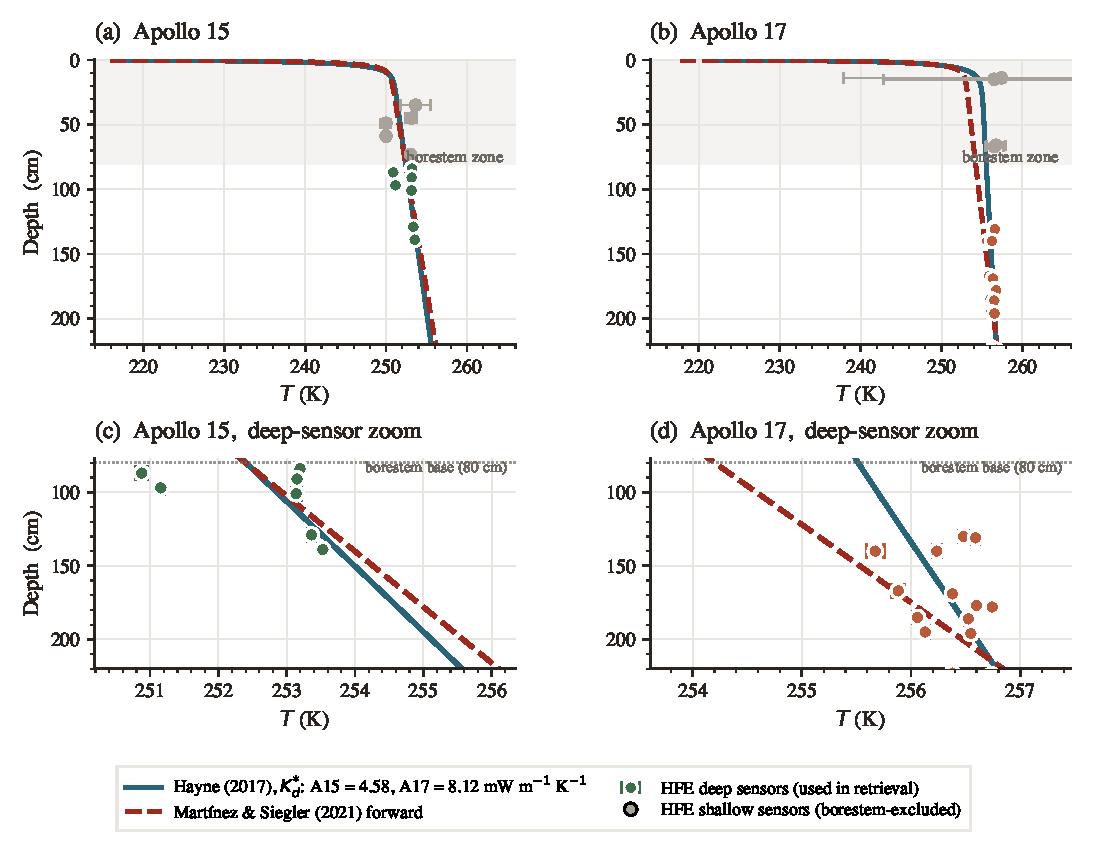
\includegraphics[width=\linewidth]{figures/fig_thermal_profiles.pdf}
\caption{\textbf{The fitted profiles.} Dots are the real deep sensors;
curves are the best-fit models. Bottom row zooms on the deep region used.
Apollo 15 shows the \emph{steeper} rise (lower conductivity needs a
steeper gradient to pass its heat); Apollo 17, more conductive, rises
more gently.}
\label{fig:profiles}
\end{figure}

\section{Why these values make physical sense}
Apollo 15's 4.6 sits between the global average (3.4) and orbital
estimates ($\sim$7), matching what the soil's fluffiness (porosity)
predicts. Apollo 17 being $\sim$1.8 times higher is explained by two
effects pointing the same way: its soil is volcanic basalt (intrinsically
more conductive than Apollo 15's highland rock), and it is slightly more
tightly packed. Neither effect needs to be extreme; together they cover
the factor of 1.8 comfortably.

\section{An independent sanity check}
The retrieval used only \emph{deep} temperatures. As a separate test, we
checked whether the same models reproduce the \emph{surface} temperature
swing measured from orbit by the Diviner instrument
(Figure~\ref{fig:diviner}). They do --- confirming the whole simulation
chain (sunlight, day length, surface balance) is set up correctly,
independently of the deep retrieval.

\begin{figure}[t]
\centering

\includegraphics[width=\linewidth]{figures/fig_diviner_closure.pdf}
\caption{\textbf{Independent check.} Grey dots: surface temperature over
a lunar day, measured from orbit. Curves: our models, which were tuned
only to the deep sensors. The good agreement confirms the setup; this
surface data was never used in the retrieval.}
\label{fig:diviner}
\end{figure}

% =====================================================================
\chapter{Honest limits and the bottom line}

A trustworthy study is clear about where it could be wrong. Ours has
three main caveats:

\begin{enumerate}
\item \textbf{Absolute values lean on the assumed $Q_b$.} Because the
      data fix the ratio $Q_b/K_d$ (the ridge of Chapter~8), revising
      the basal heat flux shifts $K_d$ proportionally. The
      \emph{difference} between sites is far more robust than either
      absolute number.
\item \textbf{Only two boreholes exist.} Two points cannot prove how
      conductivity varies across the whole Moon --- only that these two
      places differ. The broader question needs new landed missions.
\item \textbf{Apollo 17's value is systematics-sensitive.} Its error bar
      is tight, but its accuracy depends on a few input choices (like the
      surface brightness coefficient), which we report openly in the
      paper's error budget.
\end{enumerate}

\begin{keybox}
\textbf{Rock-solid:} the two sites need different conductivities, and
Apollo 17 is the more conductive one. \textbf{Conditional:} the exact
numbers, which depend on the assumed heat flux and the chosen model form.
The paper is careful, throughout, to say which is which --- and that
honesty is what makes it credible.
\end{keybox}

% =====================================================================
\appendix
\chapter{How to run the code yourself}

\begin{verbatim}
git clone https://github.com/rp3gregorio/Lunar-HFE.git
cd Lunar-HFE
python3 -m venv .venv && source .venv/bin/activate
pip install -e ".[dev]"

python scripts/pipeline/retrieve_kd.py        # the core retrieval
python scripts/figures/make_letter_figures.py # the figures
python scripts/figures/make_results_figures.py
\end{verbatim}

\noindent The pieces:
\begin{itemize}
\item \texttt{lunar/} --- the engine. \texttt{solver.py} steps the heat
      equation; \texttt{equilibrium.py} is the settled-state solver of
      Chapter~\ref{ch:bugfix}; \texttt{properties.py} holds the
      conductivity / density / heat formulas; \texttt{constants.py}
      stores every physical number with its source.
\item \texttt{scripts/pipeline/} --- the retrieval, bootstrap, Bayesian
      MCMC, AICc model comparison, and sensitivity checks.
\item \texttt{scripts/figures/} --- the figure generators, including
      \texttt{make\_book\_figures.py} and \texttt{make\_primer\_figures.py}
      which drew the teaching figures in this guidebook.
\item \texttt{output/} --- the committed results, so anyone can verify
      every number without rerunning.
\item \texttt{docs/FLAG\_REPORT.md} --- the full audit trail behind
      Chapter~\ref{ch:bugfix}.
\end{itemize}

\chapter{Glossary of every term}

\begin{description}[leftmargin=9.5em,style=nextline,font=\bfseries]
\item[Conduction] Heat spreading through solid material.
\item[Thermal conductivity ($K$, $K_d$)] How easily heat passes through
  a material; $K_d$ is the deep, settled value --- our target. Small $=$
  good insulator.
\item[Fourier's law] Heat flux $=$ conductivity $\times$ temperature
  gradient.
\item[Heat equation] The master equation: temperature changes where more
  heat flows in than out.
\item[Density ($\rho$), specific heat ($c_p$)] How much material is
  present, and how much energy it takes to warm it.
\item[Basal heat flux ($Q_b$)] The steady warmth rising from the Moon's
  interior.
\item[Gradient ($\Delta T/\Delta z$)] Degrees of temperature change per
  metre of depth. Steep $=$ good insulator (for fixed $Q_b$).
\item[Diurnal skin / skin depth] The shallow zone where the day--night
  swing is felt; the skin depth is how far it reaches.
\item[Steady state / equilibrium] The settled condition where
  temperature no longer changes from one lunar day to the next.
\item[Boundary conditions] The rules at the column's ends: radiation
  balance on top, fixed flux $Q_b$ at the bottom.
\item[Discretisation] Splitting the smooth column into thin layers and
  time into small steps so a computer can solve the equation.
\item[Borestem cut] Discarding sensors above 80\,cm because the probe
  stem contaminates them.
\item[Retrieval] Guessing $K_d$, simulating, and keeping the value that
  best matches the data.
\item[RMSE] Root-mean-square error: one number for the typical
  model--data gap, in degrees. Smaller is better.
\item[Bootstrap] Resampling your own data many times (with replacement)
  to measure how uncertain the answer is.
\item[Bayesian inference] Updating belief by combining a prior with the
  data's likelihood to get a posterior.
\item[Prior / likelihood / posterior] What you believed before / what the
  data say / the updated belief.
\item[MCMC] Markov Chain Monte Carlo: exploring all plausible answers
  with random ``walkers'' that map out the posterior.
\item[Degeneracy / ridge] When data fix only a combination of two
  unknowns (here $Q_b/K_d$), not each separately.
\item[Overfitting] A too-complex model fitting noise instead of the true
  trend.
\item[AICc] A model-comparison score: misfit plus a penalty for extra
  parameters. Lowest wins.
\item[HFE] Heat-Flow Experiment --- the Apollo instruments whose data we
  use.
\item[A15 / A17] Apollo 15 and Apollo 17 sites.
\end{description}

\end{document}
